% !TEX root = ../Planning.tex

\section{Project description (D)}
\label{sec:project-description}
\subsection{The Ampersand project}
\subsection{As-Is situation}
\subsection{Goal of the project}
\subsection{Project architecture, components and environment}
\begin{figure}[hb]
  \centering
  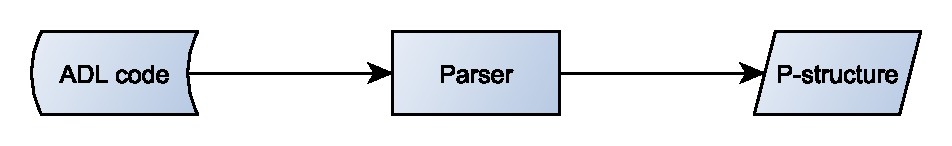
\includegraphics[width=0.5\textwidth]{Architecture}
  \caption[Architecture of the project]{Architecture of the project, showing where the parser fits in the Ampersand system}
\end{figure}

\subsection{Critical success factors}
\subsection{Our objectives and commitments towards the project and customer}

\section{Knowledge acquisition (-)}
\label{sec:knowledge-acquisition}
\subsection{Research context}
Some ideas by Bastiaan:
\begin{itemize}
  \item more info on ampersand users
  \item user-friendly error messages (specific to compilers or not)
  \item parser-libraries
  \item Stef's research (3a)
  \item Haskell parsers (e.g. Helium), monadit or combinators
\end{itemize}

\subsection{Domain \& technology}
\subsubsection{Part Daniel}
\lipsum[1]

\subsubsection{Part Maarten}
\lipsum[1]

\subsection{Knowledge documentation}
\lipsum[1]
